\subsection{Интеграция со средой разработки}
\label{sec:ide-integration}

Один из важнейших сценариев использования расширяемых и автоматизируемых программных продуктов --- возможность разработки новых скриптов и редактирование кода старых в интегрированной среде разработки.

Встроенная среда разработки как правило поставляется вместе с продуктами для автоматизации приложений, например {\it VBA} или {\it VSTA}. В платформах, основная цель которых --- поддержка плагинов, напротив, встроенных средств для редактирования кода не предоставляется. Это понятно, так как считается, что конечный пользователь не будет заниматься такой сложной задачей, как написание расширения к своему приложению. Для разработчиков же существуют отдельные пакеты (SDK) для разработки расширений в различных средах разработки.

При реализации платформы для автоматизации и расширения необходимо было предоставить удобные средства редактирования кода конечному пользователю. Эта задача может быть решена несколькими способами:

\subsubsection{Реализация собственного редактора исходного кода расширений}

Это решение имеет как и преимущества, так и целый ряд существенных недостатков. Положительным моментом этого подхода является простота интеграции в разрабатываемую платформу. Однако, реализация действительно удобного набора инструментов, таких как подсветка синтаксиса, автодополнение, автогенерация кода по шаблонам, управления файлами с исходным кодом, будет очень сложной задачей. Кроме того, результат в любом случае вряд ли сравниться с современными IDE.

\subsubsection{Использование одной из существующих IDE}

Это решение хорошо тем, что мы получаем готовую среду разработки с множеством встроенных инструментов. Однако, встает ряд вопросов, которые необходимо решить для успешного применения сторонней IDE в разрабатываемой платформе.

Интеграция в платформу. Под интеграцией необходимо понимать возможность программного управления сторонней IDE на уровне, достаточном для того, чтобы у пользователя складывалось ощущение, что он работает с единой системой, а не несколькими разными программами.

Большинство IDE обладают куда более широким, чем нужно для разработки расширений, функционалом. Поэтому важным критерием выбора сторонней IDE является ее настраиваемость и конфигурируемость. Это касается как доступных пользователю функций, так и внешнего вида самой среды.

Несмотря на предыдущий пункт, в котором сказано, что функционал современных сред разработки излишен для использования их в качестве редактора расширений, может случиться так, что некоторых специфичных функций будет нехватать. Поэтому искомая среда должна также обладать возможностью расширения функционала. Отдельным плюсом будет поддержка плагинов. Тогда можно будет отключать ненужные плагины и разработать плагины, добавляющие новый функционал.

Рассмотрим существующие среды разработки под платформу {\it .NET}.

\subsubsection{MS Visual Studio}

Удобная и мощная среда разработки от компании Microsoft. Распространяется в нескольких редакциях, различных по стоимости и функционалу. Помимо платных Professional и Ultimate версий существует бесплатная Express редакция.

Эта IDE поддерживает плагины, и имеет огромное количество разнообразных расширений, повышающих эффективность разработки.

Так же она поддерживает довольно гибкий механизм пользовательских настроек, что позволяет разработчику настроить ее <<под себя>>. Однако, отключить ненужные функции этот механизм не позволяет.

Поддерживает программное управление благодаря наличию  {\tt DTE} --- объекта верхнего уровня в объектной модели автоматизации Visual Studio. Этот объект используется для доступа к функциональности. Доступ к этому объекту осуществляется через {\tt EnvDTE} --- это обернутая сборка COM-библиотеки, содержащая объекты и члены для автоматизации ядра Visual Studio. При помощи DTE можно программно управлять средой разработки, переопределять ее поведение. Таким образом Visual Studio может быть интегрирована в платформу.

Стоит отметить, что использование DTE для управления бесплатной версией Visual Studio Express невозможно, так как в ней отсутствуют необходимые для этого компоненты.

\subsubsection{SharpDevelop}

{\it SharpDevelop} --- свободная среда разработки для {\it C\#}, {\it Visual Basic .NET}, {\it Boo}, {\it IronPython}, {\it IronRuby}, {\it F\#}, {\it C++}. Обычно используется теми, кто не хочет пользоваться {\it Visual Studio .NET}.

{\it SharpDevelop} предоставляет интегрированный отладчик, который использует собственные библиотеки и взаимодействует с исполняющей средой {\it .NET} через {\it COM Interop}.

У этой среды разработки есть ряд особенностей и преимуществ:

Во-первых, эта IDE может управляться программно извне при помощи встроенной технологии {\it SDA} {\it (SharpDevelop for Applications)}. Программное управление позволяет выполнять различные действия в IDE без участия пользователя. Например, показывать или скрывать само приложение, запускать сборку проекта, управлять сохранением и загрузкой проектов, и многие другие. 

Во-вторых, эта IDE поддерживает плагины. Это свойство позволит добавить какую-либо отсутствующую в базовой поставке функциональность не меняя исходного кода самого {\it SharpDevelop}. Это важно, так как изменение исходного кода сделает неудобным распространение готовой платформы, так как она будет совместима только с конкретной сборкой SharpDevelop. Использование плагинов позволит добавить нужную функциональность в уже установленный экземпляр этой IDE.

В-третьих, {\it SharpDevelop} поддерживает кастомизацию, то есть изменение своего внешнего вида и поведения при помощи конфигурационных файлов. Под изменением внешнего вида нужно понимать удаление <<лишних>> в контексте данного сценария использования (как внешней IDE для разработки расширений) элементов управления, добавление новых элементов управления, управление доступностью этих элементов, и прочее. Изменение поведения состоит в подмене штатных обработчиков событий элементов управления (например, кнопок), на свои собственные обработчики с измененной логикой. Например, запуск отладчика не должен пытаться стартовать сборку самого расширения (это попросту невозможно, так как расширения представляет из себя библиотеку классов), а присоединить отладчик к процессу хост-приложения.

В-четвертых, открытый исходных код поможет быстрее решить проблемы, связанные с интеграцией {\it SharpDevelop} в разрабатываемую платформу. Код IDE может быть отредактирован благодаря открытой лицензии GNU GPL v2. IDE может быть запущена под отладчиком для выявления и локализации проблем вызванных внешними факторами и нетипичным использованием самой IDE.

Наконец, она распространяется бесплатно, что делает ее очень привлекательным выбором для использования в разрабатываемой платформе.

Из недостатков этой среды стоит отметить не такой богатый инструментарий, как в VisualStudio, отсутствие аналогов многих популярных в сообществе .NET-разработчиков в среде  VisualStudio плагинов, таких как ReSharper. Не такой удобный редактор исходного кода и визуальных элементов. С другой стороны, SharpDevelop не такой <<тяжеловесный>> и потребляет мало ресурсов, что немаловажный фактор в предполагаемом сценарии его использования, как внешней среды для редактирования исходного кода расширений.

\subsubsection{MonoDevelop}

Этот продукт является кроссплатформенным форком, то есть клоном SharpDevelop, и имеет сходный с ним функционал. Более подробно рассматривать ее не имеет большого смысла. Все плюсы и минусы SharpDevelop имеют отношение и к MonoDevelop. Однако, MonoDevelop не поддерживает программное управление, в отличие от SharpDevelop, что делает SharpDevelop более предпочтительным выбором для решения поставленной задачи.

\subsubsection{Вывод}

В качестве внешней IDE для разработки расширений была выбрана IDE с открытым исходным кодом {\it SharpDevelop} (см. рисунок~\ref{pic:sharpdevelop-main-wnd}). Помимо того, что она распространяется бесплатно, имеет открытый исходный код и потребляет меньше ресурсов системы под свои нужды, инсталляционный пакет SharpDevelop имеет куда меньшие размеры, чем Visual Studio, и не содержит такое многообразие различных компонент, которые будут лишними на рабочей станции рядового пользователя ПО (не разработчика).

\begin{figure}[!h]
    \centering
    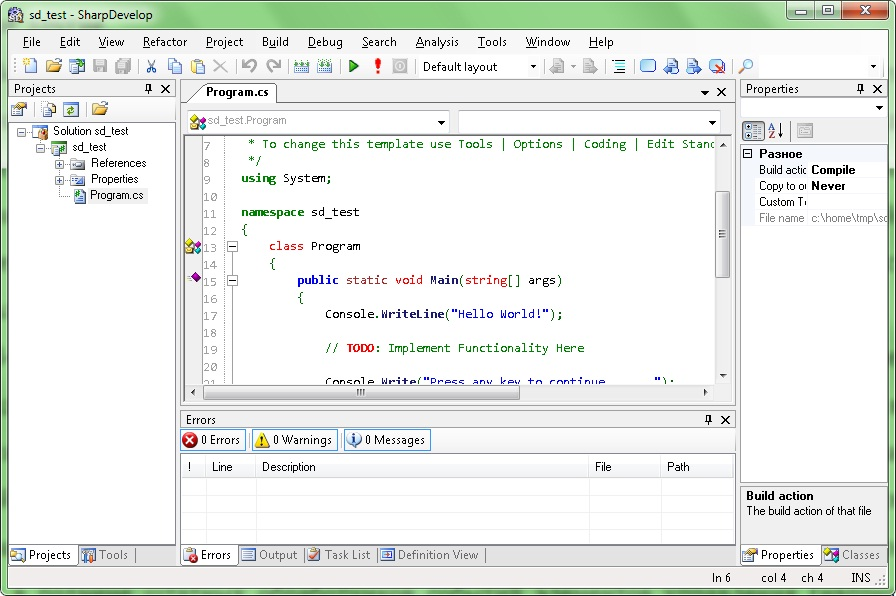
\includegraphics[width=15cm]{sharpdevelop-1.jpg}
    \caption{Основное окно SharpDevelop}
    \label{pic:sharpdevelop-main-wnd}
\end{figure} 

\pagebreak
